\definecolor{tblue}{RGB}{61,142,221}
\definecolor{torange}{RGB}{253,143,41}
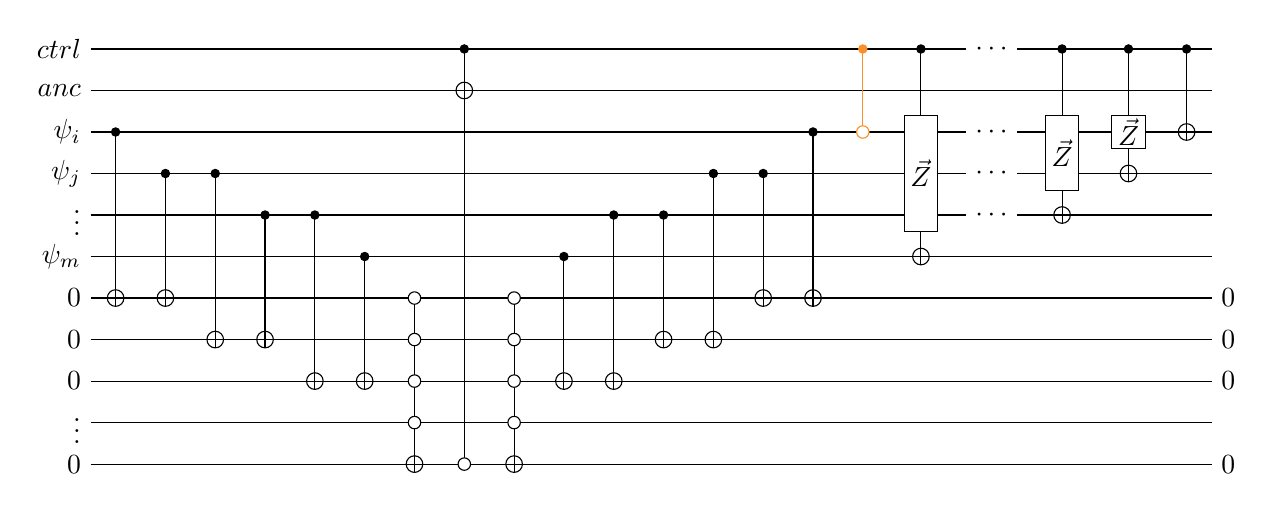
\begin{tikzpicture}[scale=1.000000,x=1pt,y=1pt]
\filldraw[color=white] (0.000000, -7.500000) rectangle (405.000000, 157.500000);
% Drawing wires
% Line 4: ctrl W ctrl
\draw[color=black] (0.000000,150.000000) -- (405.000000,150.000000);
\draw[color=black] (0.000000,150.000000) node[left] {$ctrl$};
% Line 5: anc W anc
\draw[color=black] (0.000000,135.000000) -- (405.000000,135.000000);
\draw[color=black] (0.000000,135.000000) node[left] {$anc$};
% Line 6: a W \psi_i
\draw[color=black] (0.000000,120.000000) -- (405.000000,120.000000);
\draw[color=black] (0.000000,120.000000) node[left] {$\psi_i$};
% Line 7: b W \psi_j
\draw[color=black] (0.000000,105.000000) -- (405.000000,105.000000);
\draw[color=black] (0.000000,105.000000) node[left] {$\psi_j$};
% Line 8: c W \vdots
\draw[color=black] (0.000000,90.000000) -- (405.000000,90.000000);
\draw[color=black] (0.000000,90.000000) node[left] {$\vdots$};
% Line 9: f W \psi_m
\draw[color=black] (0.000000,75.000000) -- (405.000000,75.000000);
\draw[color=black] (0.000000,75.000000) node[left] {$\psi_m$};
% Line 10: c0 W 0 0
\draw[color=black] (0.000000,60.000000) -- (405.000000,60.000000);
\draw[color=black] (0.000000,60.000000) node[left] {$0$};
% Line 11: c1 W 0 0
\draw[color=black] (0.000000,45.000000) -- (405.000000,45.000000);
\draw[color=black] (0.000000,45.000000) node[left] {$0$};
% Line 12: c2 W 0 0
\draw[color=black] (0.000000,30.000000) -- (405.000000,30.000000);
\draw[color=black] (0.000000,30.000000) node[left] {$0$};
% Line 13: 1 W \vdots
\draw[color=black] (0.000000,15.000000) -- (405.000000,15.000000);
\draw[color=black] (0.000000,15.000000) node[left] {$\vdots$};
% Line 14: c3 W 0 0
\draw[color=black] (0.000000,0.000000) -- (405.000000,0.000000);
\draw[color=black] (0.000000,0.000000) node[left] {$0$};
% Done with wires; drawing gates
% Line 16: a +c0
\draw (9.000000,120.000000) -- (9.000000,60.000000);
\filldraw (9.000000, 120.000000) circle(1.500000pt);
\begin{scope}
\draw[fill=white] (9.000000, 60.000000) circle(3.000000pt);
\clip (9.000000, 60.000000) circle(3.000000pt);
\draw (6.000000, 60.000000) -- (12.000000, 60.000000);
\draw (9.000000, 57.000000) -- (9.000000, 63.000000);
\end{scope}
% Line 17: b +c0
\draw (27.000000,105.000000) -- (27.000000,60.000000);
\filldraw (27.000000, 105.000000) circle(1.500000pt);
\begin{scope}
\draw[fill=white] (27.000000, 60.000000) circle(3.000000pt);
\clip (27.000000, 60.000000) circle(3.000000pt);
\draw (24.000000, 60.000000) -- (30.000000, 60.000000);
\draw (27.000000, 57.000000) -- (27.000000, 63.000000);
\end{scope}
% Line 18: f c0 c1 c2 c3 TOUCH
% Line 19: b +c1
\draw (45.000000,105.000000) -- (45.000000,45.000000);
\filldraw (45.000000, 105.000000) circle(1.500000pt);
\begin{scope}
\draw[fill=white] (45.000000, 45.000000) circle(3.000000pt);
\clip (45.000000, 45.000000) circle(3.000000pt);
\draw (42.000000, 45.000000) -- (48.000000, 45.000000);
\draw (45.000000, 42.000000) -- (45.000000, 48.000000);
\end{scope}
% Line 20: c +c1
\draw (63.000000,90.000000) -- (63.000000,45.000000);
\filldraw (63.000000, 90.000000) circle(1.500000pt);
\begin{scope}
\draw[fill=white] (63.000000, 45.000000) circle(3.000000pt);
\clip (63.000000, 45.000000) circle(3.000000pt);
\draw (60.000000, 45.000000) -- (66.000000, 45.000000);
\draw (63.000000, 42.000000) -- (63.000000, 48.000000);
\end{scope}
% Line 21: f c0 c1 c2 c3 TOUCH
% Line 22: c +c2
\draw (81.000000,90.000000) -- (81.000000,30.000000);
\filldraw (81.000000, 90.000000) circle(1.500000pt);
\begin{scope}
\draw[fill=white] (81.000000, 30.000000) circle(3.000000pt);
\clip (81.000000, 30.000000) circle(3.000000pt);
\draw (78.000000, 30.000000) -- (84.000000, 30.000000);
\draw (81.000000, 27.000000) -- (81.000000, 33.000000);
\end{scope}
% Line 23: f +c2
\draw (99.000000,75.000000) -- (99.000000,30.000000);
\filldraw (99.000000, 75.000000) circle(1.500000pt);
\begin{scope}
\draw[fill=white] (99.000000, 30.000000) circle(3.000000pt);
\clip (99.000000, 30.000000) circle(3.000000pt);
\draw (96.000000, 30.000000) -- (102.000000, 30.000000);
\draw (99.000000, 27.000000) -- (99.000000, 33.000000);
\end{scope}
% Line 25: -c0 -c1 -c2 -1 +c3
\draw (117.000000,60.000000) -- (117.000000,0.000000);
\draw[fill=white] (117.000000, 60.000000) circle(2.250000pt);
\draw[fill=white] (117.000000, 45.000000) circle(2.250000pt);
\draw[fill=white] (117.000000, 30.000000) circle(2.250000pt);
\draw[fill=white] (117.000000, 15.000000) circle(2.250000pt);
\begin{scope}
\draw[fill=white] (117.000000, 0.000000) circle(3.000000pt);
\clip (117.000000, 0.000000) circle(3.000000pt);
\draw (114.000000, 0.000000) -- (120.000000, 0.000000);
\draw (117.000000, -3.000000) -- (117.000000, 3.000000);
\end{scope}
% Line 26: ctrl -c3 +anc
\draw (135.000000,150.000000) -- (135.000000,0.000000);
\filldraw (135.000000, 150.000000) circle(1.500000pt);
\draw[fill=white] (135.000000, 0.000000) circle(2.250000pt);
\begin{scope}
\draw[fill=white] (135.000000, 135.000000) circle(3.000000pt);
\clip (135.000000, 135.000000) circle(3.000000pt);
\draw (132.000000, 135.000000) -- (138.000000, 135.000000);
\draw (135.000000, 132.000000) -- (135.000000, 138.000000);
\end{scope}
% Line 27: -c0 -c1 -c2 -1 +c3
\draw (153.000000,60.000000) -- (153.000000,0.000000);
\draw[fill=white] (153.000000, 60.000000) circle(2.250000pt);
\draw[fill=white] (153.000000, 45.000000) circle(2.250000pt);
\draw[fill=white] (153.000000, 30.000000) circle(2.250000pt);
\draw[fill=white] (153.000000, 15.000000) circle(2.250000pt);
\begin{scope}
\draw[fill=white] (153.000000, 0.000000) circle(3.000000pt);
\clip (153.000000, 0.000000) circle(3.000000pt);
\draw (150.000000, 0.000000) -- (156.000000, 0.000000);
\draw (153.000000, -3.000000) -- (153.000000, 3.000000);
\end{scope}
% Line 28: f +c2
\draw (171.000000,75.000000) -- (171.000000,30.000000);
\filldraw (171.000000, 75.000000) circle(1.500000pt);
\begin{scope}
\draw[fill=white] (171.000000, 30.000000) circle(3.000000pt);
\clip (171.000000, 30.000000) circle(3.000000pt);
\draw (168.000000, 30.000000) -- (174.000000, 30.000000);
\draw (171.000000, 27.000000) -- (171.000000, 33.000000);
\end{scope}
% Line 29: c +c2
\draw (189.000000,90.000000) -- (189.000000,30.000000);
\filldraw (189.000000, 90.000000) circle(1.500000pt);
\begin{scope}
\draw[fill=white] (189.000000, 30.000000) circle(3.000000pt);
\clip (189.000000, 30.000000) circle(3.000000pt);
\draw (186.000000, 30.000000) -- (192.000000, 30.000000);
\draw (189.000000, 27.000000) -- (189.000000, 33.000000);
\end{scope}
% Line 30: f c0 c1 c2 c3 TOUCH
% Line 31: c +c1
\draw (207.000000,90.000000) -- (207.000000,45.000000);
\filldraw (207.000000, 90.000000) circle(1.500000pt);
\begin{scope}
\draw[fill=white] (207.000000, 45.000000) circle(3.000000pt);
\clip (207.000000, 45.000000) circle(3.000000pt);
\draw (204.000000, 45.000000) -- (210.000000, 45.000000);
\draw (207.000000, 42.000000) -- (207.000000, 48.000000);
\end{scope}
% Line 32: b +c1
\draw (225.000000,105.000000) -- (225.000000,45.000000);
\filldraw (225.000000, 105.000000) circle(1.500000pt);
\begin{scope}
\draw[fill=white] (225.000000, 45.000000) circle(3.000000pt);
\clip (225.000000, 45.000000) circle(3.000000pt);
\draw (222.000000, 45.000000) -- (228.000000, 45.000000);
\draw (225.000000, 42.000000) -- (225.000000, 48.000000);
\end{scope}
% Line 33: f c0 c1 c2 c3 TOUCH
% Line 34: b +c0
\draw (243.000000,105.000000) -- (243.000000,60.000000);
\filldraw (243.000000, 105.000000) circle(1.500000pt);
\begin{scope}
\draw[fill=white] (243.000000, 60.000000) circle(3.000000pt);
\clip (243.000000, 60.000000) circle(3.000000pt);
\draw (240.000000, 60.000000) -- (246.000000, 60.000000);
\draw (243.000000, 57.000000) -- (243.000000, 63.000000);
\end{scope}
% Line 35: a +c0
\draw (261.000000,120.000000) -- (261.000000,60.000000);
\filldraw (261.000000, 120.000000) circle(1.500000pt);
\begin{scope}
\draw[fill=white] (261.000000, 60.000000) circle(3.000000pt);
\clip (261.000000, 60.000000) circle(3.000000pt);
\draw (258.000000, 60.000000) -- (264.000000, 60.000000);
\draw (261.000000, 57.000000) -- (261.000000, 63.000000);
\end{scope}
% Line 37: ctrl -a color=torange
\begin{scope}[color=torange]
\draw (279.000000,150.000000) -- (279.000000,120.000000);
\filldraw (279.000000, 150.000000) circle(1.500000pt);
\draw[fill=white] (279.000000, 120.000000) circle(2.250000pt);
\end{scope}
% Line 39: a b c G $\vec{Z}$ ctrl +f
\draw (300.000000,150.000000) -- (300.000000,75.000000);
\begin{scope}
\draw[fill=white] (300.000000, 105.000000) +(-45.000000:8.485281pt and 29.698485pt) -- +(45.000000:8.485281pt and 29.698485pt) -- +(135.000000:8.485281pt and 29.698485pt) -- +(225.000000:8.485281pt and 29.698485pt) -- cycle;
\clip (300.000000, 105.000000) +(-45.000000:8.485281pt and 29.698485pt) -- +(45.000000:8.485281pt and 29.698485pt) -- +(135.000000:8.485281pt and 29.698485pt) -- +(225.000000:8.485281pt and 29.698485pt) -- cycle;
\draw (300.000000, 105.000000) node {$\vec{Z}$};
\end{scope}
\filldraw (300.000000, 150.000000) circle(1.500000pt);
\begin{scope}
\draw[fill=white] (300.000000, 75.000000) circle(3.000000pt);
\clip (300.000000, 75.000000) circle(3.000000pt);
\draw (297.000000, 75.000000) -- (303.000000, 75.000000);
\draw (300.000000, 72.000000) -- (300.000000, 78.000000);
\end{scope}
% Line 40: ctrl a b c LABEL ...
\draw[color=black] (325.500000, 150.000000) node [fill=white] {$\cdots$};
\draw[color=black] (325.500000, 120.000000) node [fill=white] {$\cdots$};
\draw[color=black] (325.500000, 105.000000) node [fill=white] {$\cdots$};
\draw[color=black] (325.500000, 90.000000) node [fill=white] {$\cdots$};
% Line 41: a b G $\vec{Z}$ ctrl +c
\draw (351.000000,150.000000) -- (351.000000,90.000000);
\begin{scope}
\draw[fill=white] (351.000000, 112.500000) +(-45.000000:8.485281pt and 19.091883pt) -- +(45.000000:8.485281pt and 19.091883pt) -- +(135.000000:8.485281pt and 19.091883pt) -- +(225.000000:8.485281pt and 19.091883pt) -- cycle;
\clip (351.000000, 112.500000) +(-45.000000:8.485281pt and 19.091883pt) -- +(45.000000:8.485281pt and 19.091883pt) -- +(135.000000:8.485281pt and 19.091883pt) -- +(225.000000:8.485281pt and 19.091883pt) -- cycle;
\draw (351.000000, 112.500000) node {$\vec{Z}$};
\end{scope}
\filldraw (351.000000, 150.000000) circle(1.500000pt);
\begin{scope}
\draw[fill=white] (351.000000, 90.000000) circle(3.000000pt);
\clip (351.000000, 90.000000) circle(3.000000pt);
\draw (348.000000, 90.000000) -- (354.000000, 90.000000);
\draw (351.000000, 87.000000) -- (351.000000, 93.000000);
\end{scope}
% Line 42: a G $\vec{Z}$ ctrl +b
\draw (375.000000,150.000000) -- (375.000000,105.000000);
\begin{scope}
\draw[fill=white] (375.000000, 120.000000) +(-45.000000:8.485281pt and 8.485281pt) -- +(45.000000:8.485281pt and 8.485281pt) -- +(135.000000:8.485281pt and 8.485281pt) -- +(225.000000:8.485281pt and 8.485281pt) -- cycle;
\clip (375.000000, 120.000000) +(-45.000000:8.485281pt and 8.485281pt) -- +(45.000000:8.485281pt and 8.485281pt) -- +(135.000000:8.485281pt and 8.485281pt) -- +(225.000000:8.485281pt and 8.485281pt) -- cycle;
\draw (375.000000, 120.000000) node {$\vec{Z}$};
\end{scope}
\filldraw (375.000000, 150.000000) circle(1.500000pt);
\begin{scope}
\draw[fill=white] (375.000000, 105.000000) circle(3.000000pt);
\clip (375.000000, 105.000000) circle(3.000000pt);
\draw (372.000000, 105.000000) -- (378.000000, 105.000000);
\draw (375.000000, 102.000000) -- (375.000000, 108.000000);
\end{scope}
% Line 43: ctrl +a
\draw (396.000000,150.000000) -- (396.000000,120.000000);
\filldraw (396.000000, 150.000000) circle(1.500000pt);
\begin{scope}
\draw[fill=white] (396.000000, 120.000000) circle(3.000000pt);
\clip (396.000000, 120.000000) circle(3.000000pt);
\draw (393.000000, 120.000000) -- (399.000000, 120.000000);
\draw (396.000000, 117.000000) -- (396.000000, 123.000000);
\end{scope}
% Done with gates; drawing ending labels
\draw[color=black] (405.000000,60.000000) node[right] {$0$};
\draw[color=black] (405.000000,45.000000) node[right] {$0$};
\draw[color=black] (405.000000,30.000000) node[right] {$0$};
\draw[color=black] (405.000000,0.000000) node[right] {$0$};
% Done with ending labels; drawing cut lines and comments
% Done with comments
\end{tikzpicture}
